\PassOptionsToPackage{unicode=true}{hyperref} % options for packages loaded elsewhere
\PassOptionsToPackage{hyphens}{url}
\PassOptionsToPackage{dvipsnames,svgnames*,x11names*}{xcolor}
%
\documentclass[
]{article}
\usepackage{lmodern}
\usepackage{amssymb,amsmath}
\usepackage{ifxetex,ifluatex}
\ifnum 0\ifxetex 1\fi\ifluatex 1\fi=0 % if pdftex
  \usepackage[T1]{fontenc}
  \usepackage[utf8]{inputenc}
  \usepackage{textcomp} % provides euro and other symbols
\else % if luatex or xelatex
  \usepackage{unicode-math}
  \defaultfontfeatures{Scale=MatchLowercase}
  \defaultfontfeatures[\rmfamily]{Ligatures=TeX,Scale=1}
  \setsansfont[]{Calibri}
\fi
% use upquote if available, for straight quotes in verbatim environments
\IfFileExists{upquote.sty}{\usepackage{upquote}}{}
\IfFileExists{microtype.sty}{% use microtype if available
  \usepackage[]{microtype}
  \UseMicrotypeSet[protrusion]{basicmath} % disable protrusion for tt fonts
}{}
\makeatletter
\@ifundefined{KOMAClassName}{% if non-KOMA class
  \IfFileExists{parskip.sty}{%
    \usepackage{parskip}
  }{% else
    \setlength{\parindent}{0pt}
    \setlength{\parskip}{6pt plus 2pt minus 1pt}}
}{% if KOMA class
  \KOMAoptions{parskip=half}}
\makeatother
\usepackage{xcolor}
\IfFileExists{xurl.sty}{\usepackage{xurl}}{} % add URL line breaks if available
\IfFileExists{bookmark.sty}{\usepackage{bookmark}}{\usepackage{hyperref}}
\hypersetup{
  pdftitle={Climate Resilience Metric Report},
  colorlinks=true,
  linkcolor=Maroon,
  filecolor=Maroon,
  citecolor=Blue,
  urlcolor=blue,
  breaklinks=true}
\urlstyle{same}  % don't use monospace font for urls
\usepackage[margin=1in]{geometry}
\usepackage{graphicx,grffile}
\makeatletter
\def\maxwidth{\ifdim\Gin@nat@width>\linewidth\linewidth\else\Gin@nat@width\fi}
\def\maxheight{\ifdim\Gin@nat@height>\textheight\textheight\else\Gin@nat@height\fi}
\makeatother
% Scale images if necessary, so that they will not overflow the page
% margins by default, and it is still possible to overwrite the defaults
% using explicit options in \includegraphics[width, height, ...]{}
\setkeys{Gin}{width=\maxwidth,height=\maxheight,keepaspectratio}
\setlength{\emergencystretch}{3em}  % prevent overfull lines
\providecommand{\tightlist}{%
  \setlength{\itemsep}{0pt}\setlength{\parskip}{0pt}}
\setcounter{secnumdepth}{-2}
% Redefines (sub)paragraphs to behave more like sections
\ifx\paragraph\undefined\else
  \let\oldparagraph\paragraph
  \renewcommand{\paragraph}[1]{\oldparagraph{#1}\mbox{}}
\fi
\ifx\subparagraph\undefined\else
  \let\oldsubparagraph\subparagraph
  \renewcommand{\subparagraph}[1]{\oldsubparagraph{#1}\mbox{}}
\fi

% set default figure placement to htbp
\makeatletter
\def\fps@figure{htbp}
\makeatother


\title{Climate Resilience Metric Report}
\author{}
\date{\vspace{-2.5em}}

\begin{document}
\maketitle

\hypertarget{climate-resilience-metric-report-for-thaidene-nene-national-park-reserve}{%
\subsubsection{Climate Resilience Metric Report for Thaidene Nene
National Park
Reserve}\label{climate-resilience-metric-report-for-thaidene-nene-national-park-reserve}}

This report has been generated by the AdaptWest Climate Resilience
web-application at

\url{https://adaptwest.shinyapps.io/climate_displacement}

This report contains the data tables and figures for Thaidene Nene
National Park Reserve. Additionally, you can download the climate data
for your protected area from within the app. Additional features and
capabilities may be developed and the format of this report and the
application layout may change.

\hypertarget{introduction}{%
\subsection{Introduction}\label{introduction}}

Conservation planners and practitioners increasingly wonder how they
should revise conservation strategies in the face of the unprecedented
threat to biodiversity from climate change. One key step is to consider
the relatively consistent spatial patterns that characterize the
``geography of climate exposure and resilience''. These patterns are
often generated by the interaction of global climate systems with
regional topography, but may also be influenced by biogeographic
processes and other factors. A qualitative understanding of these
patterns can help planners craft conservation strategies that are more
resilient to uncertainty regarding the future intensity of climate
change.

The ultimate goal of landscape-level conservation planning under climate
change is to facilitate persistence of species and ecosystem processes
by increasing the adaptive capacity of landscapes and regions. The
\textbf{ESAC} framework, developed by the IPCC
\href{https://www.ipcc.ch/ipccreports/tar/wg2/pdf/wg2TARfrontmatter.pdf}{(McCarthy
et al.~2001)}, proposes that climate Exposure and Sensitivity interact
and are mediated by Adaptive Capacity, resulting in the degree of
vulnerability of the system to climate change.

Most of the data considered here are measures of climate
\textbf{exposure}. Data, such as the location of climate refugia for
individual species, which incorporates information on a species'
climatic tolerances or niche, also addresses climate
\textbf{sensitivity}. The ultimate goal of providing such information to
planners is to support conservation management that, by protecting key
areas identified by the data, increases the \textbf{adaptive capacity}
of the landscape and its ability to support native species and
ecosystems into the future.

A diversity of conservation strategies is needed to address climate
change adaptation challenges. Among the most important are
identification and protection of climate refugia (areas buffered from
climate change where organisms can persist) and climate corridors (areas
that play a key role in facilitating dispersal under climate change).

For further information and citation refer to:

Carroll, C. \& Noss, R. F. (2020) Rewilding in the face of climate
change. Conservation Biology in press.
\href{http://dx.doi.org/\%5Bdoi\%5D}{doi: 10.1111/gcb.13663}.

\pagebreak

In this report, we present data for on key metrics that can be used to
assess landscape-level climate resilience and vulnerability. Spatial
data shown in this report are freely available at the links below.

\textbf{Climate Resilience Metric:}

\begin{itemize}
\tightlist
\item
  \href{https://adaptwest.databasin.org/pages/adaptwest-velocitywna}{Forward
  and backward climatic velocity}
\item
  \href{https://adaptwest.databasin.org/pages/environmental-diversity-north-america}{Topodiversity}
\item
  \href{https://adaptwest.databasin.org/pages/climatic-macrorefugia-for-trees-and-songbirds}{Biotic
  velocity}
\item
  \href{https://adaptwest.databasin.org/pages/climate-connectivity-north-america}{Climate
  connectivity}
\item
  \href{http://globbiomass.org/wp-content/uploads/GB_Maps/Globbiomass_global_dataset.html}{Aboveground
  forest carbon}
\item
  \href{https://data.isric.org/geonetwork/srv/eng/catalog.search\#/metadata/c02ddf8b-cbfb-4533-a9c3-7bf0790fd042}{Soil
  carbon}
\item
  \href{https://figshare.com/articles/Global_Human_Modification/7283087}{Intactness
  (the inverse of landuse intensity)}
\end{itemize}

\hypertarget{basic-information-for-thaidene-nene-national-park-reserve}{%
\subsection{Basic Information for Thaidene Nene National Park
Reserve}\label{basic-information-for-thaidene-nene-national-park-reserve}}

Adaptation Metrics for: Thaidene Nene National Park Reserve

Intactness

Topodiversity

Forward Climatic Refugia

Backwards Climatic Refugia

Bird Refugia

Tree Refugia

Tree Carbon

Soil Carbon

Name

9

0.9990

32.4678

1.0540

0.9747

0.2091

0.0033

17.2688

458.3263

L1\_EcoRegion\_9

0.9984

72.4476

1.0256

0.8759

0.1865

0.0606

28.5343

373.2780

L2\_EcoRegion\_32

0.9994

35.0552

0.9624

0.8727

0.2233

0.0564

21.5761

381.3357

L3\_EcoRegion\_84

0.9994

31.4958

1.1487

0.8932

0.1585

0.0208

24.3071

391.6957

\hypertarget{land-cover-classification-for-thaidene-nene-national-park-reserve}{%
\subsection{Land Cover Classification for Thaidene Nene National Park
Reserve}\label{land-cover-classification-for-thaidene-nene-national-park-reserve}}

The table below summarizes the 2010 MODIS Landcover Classification 250
dataset produced by Natural Resources Canada/ The Canada Centre for
Mapping and Earth Observation (NRCan/CCMEO), United States Geological
Survey (USGS); Insituto Nacional de Estadistica y Geografia (INEGI),
Comision Nacional para el Conocimiento y Uso de la Biodiversidad
(CONABIO) and Comisipn Nacional Forestal (CONAFOR).

{[}1{]} ``WE NEED TO PRECALCULATE THIS SO IT IS FAST. ALSO WE SHOULD
UPDATE TO NEWER\nVERSION'' \#\#\# Organizations participating in or
supporting development of the application: AdaptWest, Canadian Forest
Service

\pagebreak

\hypertarget{map-of-forwards-climate-refugia-for-thaidene-nene-national-park-reserve}{%
\subsection{Map of forwards climate refugia for Thaidene Nene National
Park
Reserve}\label{map-of-forwards-climate-refugia-for-thaidene-nene-national-park-reserve}}

\begin{center}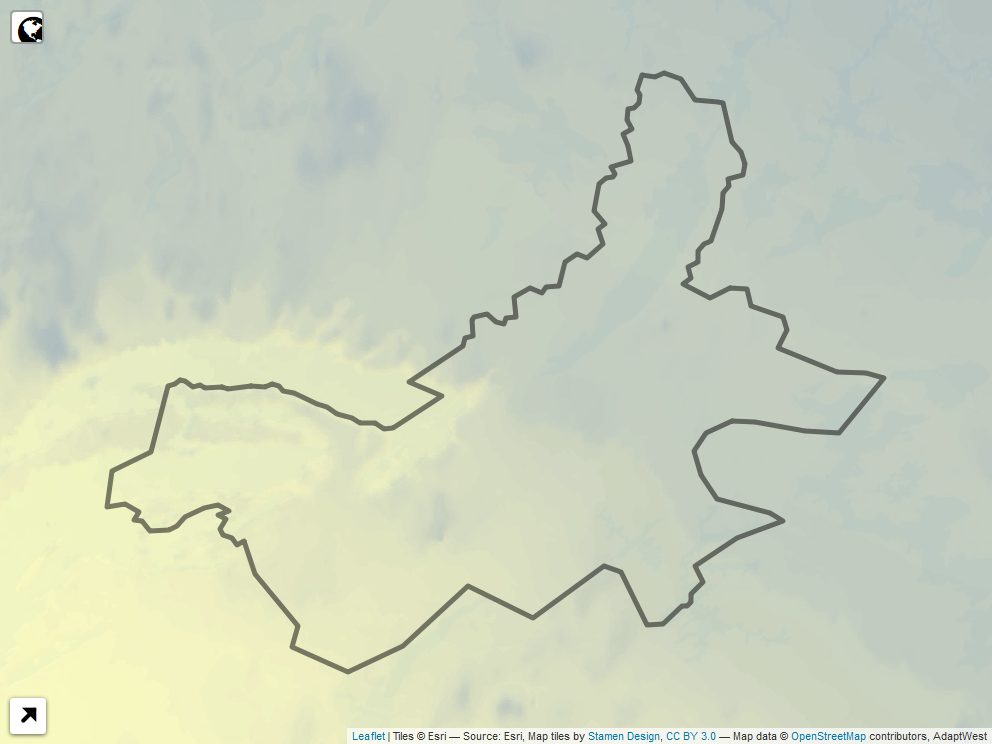
\includegraphics[width=0.7\linewidth]{./fwsvel} \end{center}

\textbf{Climate velocity} is the speed that an organism needs to travel
to keep pace with climate. Climate refugia (areas of species persistence
during climate change) are areas of low enough velocity that the
organism can remain within their suitable climate.

To calculate analog-based climatic velocity, climate is categorized into
types, and the straight-line distance is measured between a site and the
nearest site with the same climate type in a different time period.
Climatic velocity is influenced by processes at several scales:

\begin{itemize}
\tightlist
\item
  Local topography
\item
  Regional topographic position
\item
  Location on continent
\item
  Location in relationship to global climate circulation patterns
\end{itemize}

\textbf{Forward climatic velocity} measures the straight-line distance
between a site's current climate type and the nearest site with the same
climate type under future climates. This represents the rate at which an
organism currently at a location must move to find future suitable
climate.

The map above shows refugia based on forward climatic velocity from
current to 2080s climate for a ``business-as-usual'' emissions scenario
(RCP8.5).

\pagebreak

\hypertarget{map-of-backwards-climate-refugia-for}{%
\subsection{Map of backwards climate refugia
for}\label{map-of-backwards-climate-refugia-for}}

\textbf{Backward climatic velocity} measures the straight-line distance
between a site's future climate type and the nearest site with the same
climate type under current climates. This represents the rate at which
organisms adapted to a location's future climate will need to move to
colonize that location. Backward velocity represents the distance and
rate at which organisms adapted to a location's future climate will need
to move to reach that location, and reflects a location's ability to
serve as a refugium for species and ecosystems. Backward velocity is
generally low in alpine areas, because adapted organisms can reach the
site from nearby downslope locations. Values are often high in valley
bottom habitat because organisms must travel longer distances to
colonize these locally new habitat conditions.

Areas with low backward climatic velocity will have higher values as
refugia, so we transform velocity values to a refugia index by
multiplying the log transformation of velocity by negative 1. A log
transformation is used because we are most interested in variation in
the index at relatively low velocity values.

The map above shows refugia based on backward climatic velocity from
current to 2080s climate for a ``business-as-usual'' emissions scenario
(RCP8.5).

\pagebreak

\hypertarget{map-of-microrefugia-potential-for}{%
\subsection{Map of Microrefugia Potential
for}\label{map-of-microrefugia-potential-for}}

\textbf{Microrefugia potential} - Many approaches to identifying areas
that will be refuges for biodiversity under climate change are based on
predicting future climate. Other approaches use only information on the
current environment. Species distributions, communities, ecosystems, and
broader patterns of biodiversity are known to be influenced by abiotic
drivers such as soils, geology, and topography. Refugia also span a
range of spatial scales. Coarse-resolution metrics such as climatic
velocity which identify \textbf{macrorefugia} (areas where broad-scale
climate is relatively stable and suitable for persistence) can be
complemented with other information that helps identify fine-scale
\textbf{microrefugia} (small areas with locally favorable environments
within otherwise unsuitable climates).\\
Micro-scale climate refugia can be created by terrain-related factors,
as shown in the figure below from
\href{https://journals.plos.org/plosone/article?id=10.1371/journal.pone.0159909}{Morelli
et al.~(2016).} Topographic diversity (topodiversity) data are useful
for identifying areas where a heterogeneous physical environment (e.g.,
steep elevation gradients or diverse aspects) increases the likelihood
that species will be able to find nearby suitable habitat as climate
changes.\\
Microrefugia occur both within and outside of macro-refugia (areas of
lowest climate velocity).\\
The map above shows topographic diversity. The spatial data can be
downloaded
\href{https://adaptwest.databasin.org/pages/environmental-diversity-north-america}{here}.

\pagebreak

\hypertarget{map-of-biotic-velocity-for}{%
\subsection{Map of Biotic Velocity
for}\label{map-of-biotic-velocity-for}}

\textbf{Biotic velocity} is a metric that combines data from climate
projections with data on the distributions of individual species.
Climatic niche models based on correlations between species
distributions and current climatic conditions are then projected forward
to predict distribution under future climates. Biotic velocity
represents the distance between a site and the nearest site projected to
be climatically suitable for the species under future projected
climates.\\
Biotic velocities provide a lower estimate of migration requirements
than does climatic velocity because the metric assumes local populations
can adapt to any climatic conditions found within the full range of the
species current distribution. The metric can be reported on a
per-species basis or averaged across a taxa group. Backward biotic
velocity provides a species-specific refugia index. When compared to
refugia defined by low climatic velocity, biotic velocity highlights the
influence of biogeographic factors (including past refugia locations)
which have made certain regions, such as California and the southern
Appalachians, more biodiverse than expected based on climate alone.
Biotic-velocity-based refugia vary depending on the species considered.
Stralberg et al.~2018 mapped refugia for 592 songbird and tree species.
The map above shows refugia based on climatic niche models for songbirds
(left panel) and trees (right panel). The spatial data can be downloaded
\href{https://adaptwest.databasin.org/pages/climatic-macrorefugia-for-trees-and-songbirds}{here}.

\pagebreak

\hypertarget{map-of-climate-connectivity-for}{%
\subsection{Map of Climate Connectivity
for}\label{map-of-climate-connectivity-for}}

\textbf{Climate connectivity} - The persistence of many species under
climate change will depend areas that facilitate dispersal to newly
climatically suitable habitat. \textbf{Climate connectivity areas} or
``climate corridors'' are areas that form the best route between current
climate types and where those climates will occur in the future under
climate change. Climate connectivity areas are distinct from refugia and
thus poorly captured by many existing conservation strategies. Because
dispersing organisms may need to avoid hostile climates, these routes
are often circuitous rather than the straight-line paths, as is assumed
when measuring standard climatic velocity
\href{https://www.nature.com/articles/ncomms12349}{Dobrowski and Parks
2016}. Several methods exist for identifying climate corridors.
\href{https://onlinelibrary.wiley.com/doi/full/10.1111/gcb.14373}{Carroll
et al.~2018} used centrality metrics to identify areas where many
potential dispersal paths overlap. Broad-scale topography and climate
influence connectivity paths. Routes were found to be funneled along
north-south trending passes and valley systems and along the leeward or
drier slopes of north-south trending mountain ranges. Climate
connectivity paths also tend to avoid areas of novel and disappearing
climates. Human landuses may further constrain the ability of species to
disperse through these areas. The map above shows forward (left panel)
and backward (right panel) climatic connectivity areas from current to
2080s climate for a ``business-as-usual'' emissions scenario (RCP8.5).
The spatial data can be downloaded
\href{https://adaptwest.databasin.org/pages/climate-connectivity-north-america}{here}.

\pagebreak

\hypertarget{map-of-above--and-below-ground-carbon-for}{%
\subsection{Map of Above- and Below-Ground Carbon
for}\label{map-of-above--and-below-ground-carbon-for}}

\textbf{Above- and below-ground carbon} - Climate adaptation planning
addresses the impacts of climate change via efforts to increase
landscape resilience and other strategies. However, it is important to
place climate adaptation strategies within a larger context which
includes mitigation strategies to address the causes of climate change
by reducing accumulation of greenhouse gases in the atmosphere. An
example of such a dual adaptation/mitigation strategy is a recent
conservation proposal termed the Global Deal for Nature, which proposes
that protected area networks be expanded to include areas that hold
large reserves of \textbf{aboveground (biomass) and belowground (soil
and biomass) carbon}, with the aim of reducing disturbances that
accelerate release of stored carbon
(\href{http://doi.org/10.1126/sciadv.aaw2869}{Dinerstein et al.~2019}).
In North America, soil carbon is generally at highest levels in large
boreal peatlands, implying that protection of large boreal landscapes is
critical for conserving areas of high soil carbon. Patterns of
above-ground carbon are complex and vary based on several broad-scale
climatic and other factors. A strong longitudinal precipitation gradient
is evident in North America, as predominantly west-to-east atmospheric
circulation interacts with north-south cordilleras such as the Rocky
Mountains. More mesic forested ecosystems to the west of these ranges
generally support higher levels of aboveground carbon in terms of tree
biomass. Grassland ecosystems can also support high levels of
belowground carbon. The map above shows above-ground carbon stored in
tree biomass (left panel) and below-ground soil carbon (right panel).
The spatial data can be downloaded
\href{http://globbiomass.org/wp-content/uploads/GB_Maps/Globbiomass_global_dataset.html}{here}
and
\href{https://data.isric.org/geonetwork/srv/eng/catalog.search\#/metadata/c02ddf8b-cbfb-4533-a9c3-7bf0790fd042}{here}.

\pagebreak

\hypertarget{map-of-intactness-for}{%
\subsection{Map of Intactness for}\label{map-of-intactness-for}}

\textbf{The Human Footprint} - The effects of climate stressors on
natural systems interact with and can be magnified by other human-caused
stressors such as land conversion and development. Human modification of
the landscape shows a strong latitudinal gradient in North America,
increasing in intensity from the boreal region to mid-latitudes. In much
of the boreal region, development corridors are embedded within a more
intact matrix. In mid-latitude regions, large protected area complexes
and other wild areas appear as islands within a more developed matrix.
The intensity of anthropogenic stressors has been termed the
\textbf{human footprint} or \textbf{human modification index}
(\href{https://onlinelibrary.wiley.com/doi/abs/10.1111/gcb.14549}{Kennedy
et al.~2019}). We represent this metric here as intactness, the inverse
of anthropogenic landuse intensity, so that, as with other climate
resilience metrics described here, increasing values of the metric
correspond to increasing resilience. The figure below shows the specific
data used by
\href{https://onlinelibrary.wiley.com/doi/abs/10.1111/gcb.14549}{Kennedy
et al.~2019} to produce a composite human modification index. The map
above shows intactness (the inverse of human land use intensity). The
spatial data can be downloaded
\href{https://figshare.com/articles/Global_Human_Modification/7283087}{here}.

\pagebreak

\hypertarget{climate-resilience-metric-star-plot-for}{%
\subsection{Climate Resilience Metric Star Plot
for}\label{climate-resilience-metric-star-plot-for}}

\textbf{Data visualization} - The wide variety of climate exposure and
refugia metrics can seem confusing. However, there are several ways to
integrate information from diverse metrics. As discussed previously,
coarse-resolution velocity metrics can be combined with fine-resolution
diversity metrics in order to leverage the respective strengths of the
two groups of metrics as tools for identification of potential macro-and
microrefugia that in combination help maximize both transient and
long-term resilience to climate change. Alternately, planners can
integrate multiple climate exposure metrics for an area of interest into
a single diagram to produce a composite ``fingerprint'' representing
factors affecting climate resilience.
\href{http://science.sciencemag.org/content/344/6183/1247579}{Garcia et
al.~2014} developed the concept of using a star plot to show the varying
magnitudes of different climate metrics. A star plot provides a compact
way to communicate contrasts between the intensity of different climate
exposure stressors in a region. The figure above compares starplot
patterns for 9 major protected area complexes within the
Yellowstone-to-Yukon (Y2Y) region. The contrast in starplot patterns
between southern (e.g., Yellowstone) and northern (e.g., Nahanni)
protected areas within Y2Y reflects the long-noted dichotomy between
centers of species diversity (hotspots) and wild landscapes (coldspots).
Northern protected areas within Y2Y score highly in intactness and
protection of soil carbon, whereas southerly protected areas play a
greater role in providing macrorefugia as defined by both species models
and climatic velocity. For more information on patterns of climate
resilience within North American protected areas, see this app's
\textbf{Protected Area Tour} tab. To view and compare maps of climate
resilience metrics, see this app's \textbf{Climate Resilience Metrics
Explorer} and \textbf{Protected Area Explorer} tabs.

\hypertarget{climate-resilience-metric-scatterplots-for}{%
\subsection{Climate Resilience Metric Scatterplots
for}\label{climate-resilience-metric-scatterplots-for}}

\textbf{Minimal descriptive text} - To create and compare scatterplots
of climate resilience metrics, see this app's \textbf{Climate Resilience
Metrics Explorer} and \textbf{Protected Area Explorer} tabs.

\end{document}
